\section{Implementation}
\label{implementation}

The AI4Agile app was implemented within Jira Cloud as an app and connected to a Python-based backend. Table \ref{tab:tools} shows a summary of the tools we have investigated and/or adopted to implement the various components and subcomponents in the system. A further detailed breakdown of the implementation follows in the subsections below.

%\begin{center}
\begin{table}
\centering
\caption{Components, subcomponents, and sources used for implementation of subcomponents}
\label{tab:tools}
\begin{tabular}{ |c|c|c| } 
\hline
\multicolumn{1}{|c|}{\textbf{Component}} & \multicolumn{1}{c|}{\textbf{Subcomponent}} & \multicolumn{1}{c|}{\textbf{Source}} \\
\hline
Epic Decomposition & K-means clustering & scikit-learn: machine learning in Python \cite{scikit} \\
\hline
\multirow{4}{*}{Story Optimization} & Word embedding & scikit-learn: machine learning in Python \cite{scikit} \\ 
\cline{2-3}
& Feature Extraction & scikit-learn: machine learning in Python \cite{scikit} \\ 
\cline{2-3}
& Cosine similarity & scikit-learn: machine learning in Python \cite{scikit} \\
\cline{2-3}
& Function decision & N/A \\ 
\hline
\multirow{2}{*}{Task Generation} & Sentence classification & Stanford CoreNLP \cite{NLP1, stanza} \\ 
\cline{2-3}
& Part of speech tagging & Natural Language ToolKit \cite{nltk} \\ 
\hline
\multirow{3}{*}{UI} & Tree relationship graph & Cytoscape \cite{cytoscape} \\ 
\cline{2-3}
& Clustered relationship graph & Cytoscape \cite{cytoscape} \\ 
\cline{2-3}
& Jira Cloud frontend & Atlassian Connect Express Modules \cite{jiraconnect}\\ 
\hline
\end{tabular}
\end{table}
%\end{center}

\subsection{Frontend}

As part of the Atlassian Design Guidelines\cite{jira3}, a frontend library, Atlassian User Interface (AUI)\cite{jira4}, is provided to create new UI elements to match Jira’s style and user experience. The team coded our own UI components adhering Design Guidelines from Atlassian.

Within Jira, all objects (epics, stories, issues) are rendered in the same way, each containing a shared issue panel as shown in Fig. \ref{fig:issueView}. Our app is implemented within the issue panel in the form of additional panels that can be opened through added buttons. When a process button or visualization button is pressed, a new panel appears.

Each of the processes uses the same suggestion panel, with variations depending on the need for user inputs in the case of epic decomposition and story optimization. The suggestion panel, when opened, requests suggestions from the backend through jQuery AJAX\cite{ajax} and displays a loading animation until the suggestions are received. Stories can be changed and once checked, they can be created which is done by passing the selected stories via an AJAX call to the backend. The responsibility to populate selected stories to the Jira board is handled by the backend.

\begin{figure}
\centering
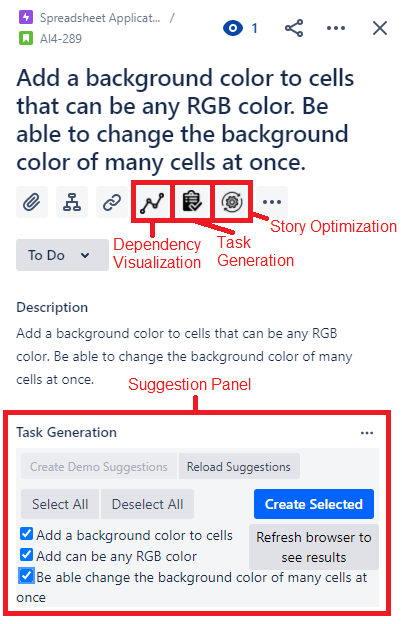
\includegraphics[width=.5\textwidth,keepaspectratio]{./figure/Frontend.png}
\caption{Issue Panel within Jira with Task Generation suggestions }
\label{fig:issueView}
\end{figure}

\subsection{Backend}

The backend served two primary purposes: generating suggested issues and populating selected suggestions into Jira. Each process has its corresponding suggestion generator and selected suggestion creator since the specifics of each type of issue varies. Jira handles all issue types (i.e. epics, stories, and tasks) in the same manner, each having an identical set of shared fields with the addition of customized fields depending on the type of issue.

All three processes were implemented using available Python libraries, with the primary interface also written in Python. The interface uses Flask\cite{flask}, a Python web framework, to receive messages sent by AJAX in the frontend. The AI interface component uses atlassian-Python-api\cite{jiraPython}, which simplifies Atlassian Rest API\cite{jira5} calls, to gather necessary information from the Jira issues. When generating suggestions, the description is queried for and passed as a list of individual requirements to the text processor. Suggestions are then passed back through a reply to the original message. Once a user selects, and possibly edits, which issues they would like to have populated in their Jira board, then the original issue is queried again to percolate existing fields, such as assignee, reporter, due date, tags, or sprints, to the newly created child issues. Each newly created issue is given a blocking relationship to the issue they were derived from. For example, all the created stories from an Epic Decomposition will “block” the epic from being completed. Any further tasks created from Task Generation on a story will “block” the story from completion.

\subsubsection{Epic Decomposition}

The Epic Decomposition process was implemented using k-means clustering over a dynamic clustering technique, such as DBSCAN or Mean shift. Dynamic clustering techniques were unable to be implemented in a manner that yielded consistent meaningful clusters across many epic inputs. This was a result of an inability to filter noises such that the clusters were neither completely disjoint nor entirely overlapping. Thus, K-means, a centroid-based clustering algorithm, was used at the cost of selecting a default number of stories to generate. The default number of stories generated is five, but the user can select between two and ten stories using a newly added slider in the UI for the Epic Decomposition process.

\subsubsection{Story Optimization}
For Story Optimization, in the beginning, a pre-trained Word2Vec model was used to extract the features out of sentences. A sentence embedding technique called SIF embeddings (Smooth Inverse Frequency) was used to compute sentence embeddings as a weighted average of word vectors. However, these techniques were extremely computationally intensive. The story optimization also required every sentence to be compared against one another, which led to a long waiting time. To overcome the obstacle, the implementation was changed to use TF-IDF from the scikit-learn python library. The technique was also able to extract features from sentences with a faster process time.

Initially, the degree of connectivity between sentences was specified by choosing the optimal threshold level. However, it was changed so that the user can choose to increase or decrease the degree of connectivity between sentences offering more flexibility in the generated results.

The user can choose to increase or decrease the degree of connectivity between sentences. The slider displays options from 0 to 10, which maps to values from 0.65 to 0.75 as threshold values on the backend. The slider integration was a feature that was added based on mentor feedback. A parameter is exposed to give the user more control of the output. The exposed parameter is the degree of connectivity between the sentences. It was determined after impact analysis that it is better to implement it this way because it generates more meaningful results tailored to each user. This also eliminates the need for having a fixed threshold number, since the optimal threshold number can vary between inputs.

\subsubsection{Task Generation}
The approach for Task Generation was based off a decomposition approach by Das, Majumder, and Phadikar in 2018 \cite{NLP1}. We initially selected the natural language toolkit (NLTK) library \cite{nltk} to implement the task generation function, but it did not satisfy our need for parts-of-speech tagging as the library lacked the word dependency feature. Word dependency is necessary to our process for generating simple sentences by returning a pair of words while identifying the dependency between them. Hence we switched to a new Python NLP library Stanza \cite{stanza} derived as part of the research presented in \cite{NLP1}. This library allows for parts-of-speech tagging, word dependency, and tree parsing. By having part-of-speech tagging and word dependency, the creation of simple sentences from complex and compound sentences was easier to implement.

\subsection{Communication}
\begin{figure}
\centering
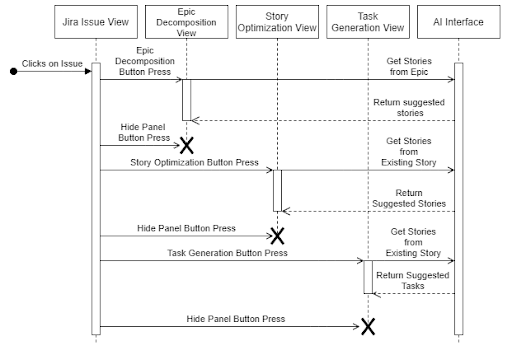
\includegraphics[width=0.75\textwidth,keepaspectratio]{./figure/SequenceFlowDiagram.png}
\caption{Suggestion web panel sequence diagram of messages between the frontend Jira web page and AI4Agile backend}
\end{figure}

The plugin communicates from Jira to the backend interface via a listener through AJAX calls which are received by Flask. When a web panel is opened for any of the three processes, a message is sent to generate and return the suggestion issues. The Jira panel will function asynchronously with a loading animation appearing until the resulting suggestions are received. Once the results are received, populated in the suggestion box, and the desired suggestions are selected by the user, then a message is sent containing which suggestions to then create within Jira.

\subsection{Hosting}
\label{hosting}

The AI4Agile Jira Connect App frontend and backend is hosted as three Azure Web Apps. The frontend is a single Node.js Web App and the backend consists of two Python Web Apps. As previously discussed, the frontend uses AJAX and the backend uses Flask Web Framework for communication. Jira communicates with the frontend Azure Web App to get assets that are to be rendered within Jira. The backend is separated into two sets of features: dependency visualization and text processing. The dependency visualization backend accesses the data from Jira, which is used to construct graphs. The text processing backend contains all three of the primary processes (epic decomposition, story optimization, and task generation). The Jira web page does not directly communicate with the backend. Rather, the Jira web page communicates with the frontend and then the frontend communicates with the backend. The flow of communication between AI4Agile's frontend and backend web apps, along with the Jira web page is  shown in Fig. \ref{fig:hostingRelationship}

\begin{figure}
\centering
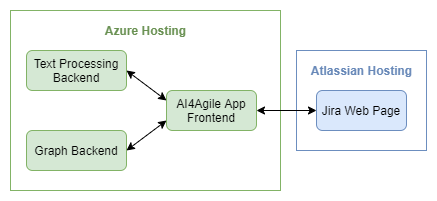
\includegraphics[width=0.75\textwidth,keepaspectratio]{./figure/hostingRelationship.png}
\caption{Relationship between AI4Agile Web Apps and Jira}
\label{fig:hostingRelationship}
\end{figure}